%
% ---------------------------------------------------
%
% Trabajo de Final de Grado:
% Author: Gonzalo Jesús García Martín <dracoyue@gmail.com>
% Capítulo: Objetivos
% Fichero: Cap4_Antecedentes.tex
%
% ----------------------------------------------------
%

\cleardoublepage
\chapter{Antecedentes}
\label{chap:record}

	Con los nuevos avances tecnológicos se ha vuelto popular el uso de las comúnmente denominada {\it apps} en los dispositivos móviles. Hay aplicaciones para todos los gustos, desde lo más básico como aprender a cocinar o aplicaciones de comunicación, hasta de lo más importante como por ejemplo consultar la información de la cuenta del banco e incluso hacer operaciones con ella.
	
	\bigskip
	Se ha observado que en el ámbito docente hay una falta de comunicación entre padres y profesores. También el aumento de problemas como el acoso, fracaso escolar o incluso problemas de ámbito familiar influyen en los alumnos. Por eso los hasta ahora recursos tradicionales no eran suficientes. Notas escritas y reuniones no son más que informes puntuales de un progreso continuo que puede decaer sin aviso previo.
	
	\bigskip
	Por eso se presenta una herramienta que intenta establecer un flujo de información continua sin comprometer los datos personales de los usuarios tales como el teléfono o el correo. Así éstos se sentirán cómodos a la hora de comunicarse de forma segura. Se entiende que es un esfuerzo extra para los equipos docentes, pero permitirá que haya una mejor comunicación para resolver problemas inesperados y actuar de forma casi inmediata.
	
	\section{Otras Aplicaciones similares}
	
	A continuación se describirán aplicaciones similares a la que se ha desarrollado.
	
	\subsection{Remind}
	{\it Remind}\cite{3:remind:online} ofrece a los usuarios una forma sencilla de comunicación segura ya que los números de teléfono se mantienen confidenciales. Administradores o personal docente se pueden comunicar con los estudiantes y padres de forma personal, con un chat, o de forma generalizada enviando anuncios.
	
	\bigskip
	El profesor creará una o varias clases y obtendrá un código por cada clase que cree. Con este código los padres y alumnos podrán apuntarse a sus clases, recibiendo notificaciones o mensajes de los profesores, monitores y administradores. 
	
	En la figura \ref{fig:Remind} se puede apreciar la pantalla de bienvenida.
	
	\begin{figure}[h !]
		\centering
		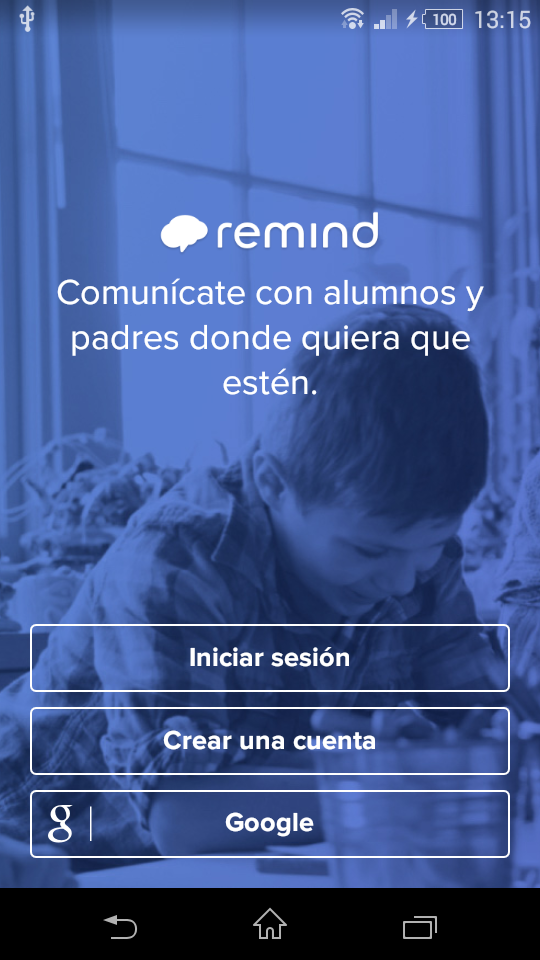
\includegraphics[scale=0.2]{Remind}
		\caption{Pantalla Bienvenida de la Aplicación Remind}
		\label{fig:Remind}
	\end{figure}
	
	\subsection{miColegioApp}
	En {\it miColegioApp}\cite{4:micolegioapp:online} el usuario se registra como alumno, profesor, padre, madre, tutor legal o persona autorizada. Una vez registrado, se solicita el código al centro, que debe haber contratado los servicios de la empresa previamente, y se introduce en la aplicación. Cuando se ha asociado al usuario con un centro, el dueño del dispositivo recibirá notificaciones y circulares del colegio.
	En la figura \ref{fig:miColegioApp} se observa la pantalla de inicio.
	
	\begin{figure}[h !]
		\centering
		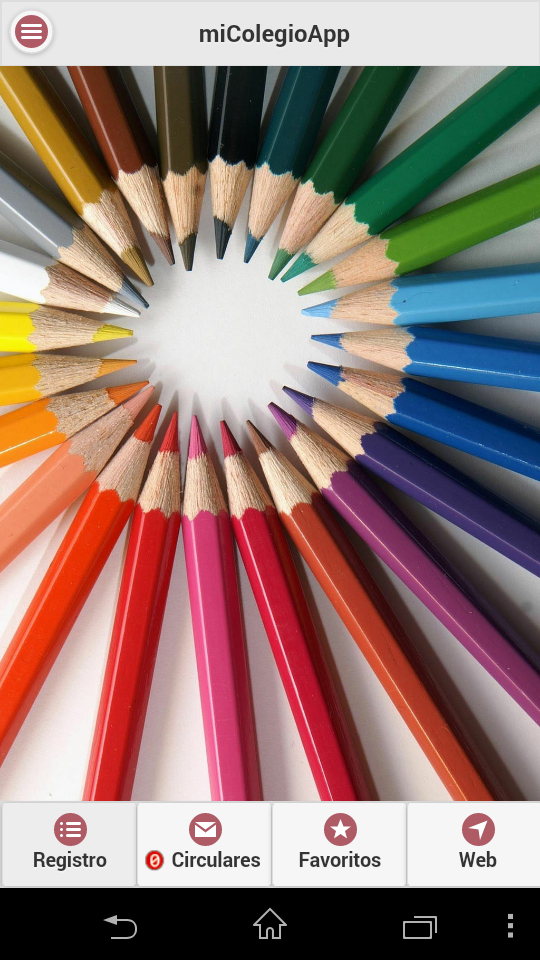
\includegraphics[scale=0.2]{miColegioApp}
		\caption{Pantalla Bienvenida de la Aplicación miColegioApp}
		\label{fig:miColegioApp}
	\end{figure}